\subsubsection{Semaphore}
\begin{figure}[h]
\centering
\nogloxy{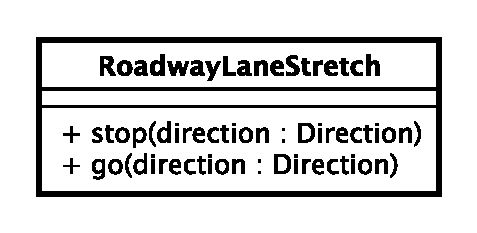
\includegraphics[scale=0.6,keepaspectratio]{diagrams/workspace/application/roadwayLaneStretch.eps}}
\caption{Application::RoadwayLaneStretch}
\end{figure}
\FloatBarrier
A semaphore is placed at the end of a roadway lane stretch offers the following operations:
\begin{itemize}
	\item \texttt{stop(direction : Direction)}
	\\Blocks outgoing flow of vehicles going towards a given direction
	\item \texttt{go(direction : Direction)}
	\\Allows outgoing flow of vehicles going towards a given direction
\end{itemize}
\paragraph{Remaks}
\ \\\texttt{stop} and \texttt{go} operations are called by a set of semaphores, that communicate internally to advance through their RGY steps.

The \texttt{direction} parameter assumes the values:
\begin{itemize}
	\item N or S  for “vertical” street
	\item W or E for “horizontal” street
\end{itemize}